\section{第2讲\quad 几何}

\item {
    【巧求周长·平移】
    图中的八边形是将大长方形纸片剪去一个小长方形得到.则至少需要知道(\quad)条线段的长度, 才可以计算出这个八边形的周长. \\
    {A.4\qquad B.3\qquad C.5\qquad D.10}
    \begin{figure}[H] 
        \centering
        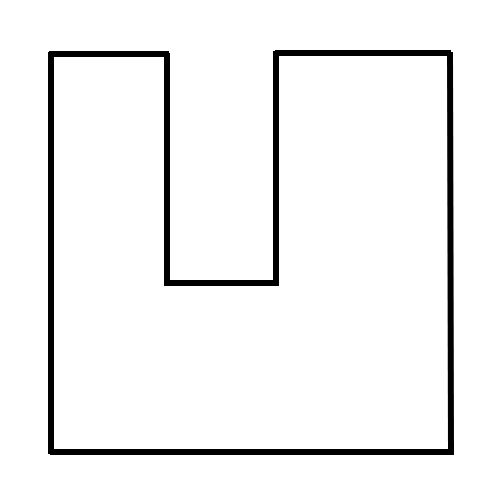
\includegraphics[width=0.3\textwidth]{./pics/Chapter_2/14.png}
    \end{figure}
    \ifshowSolution 
        \fangsong\zihao{5}\textcolor{blue}{
            正解: 平移法.至少需要知道3条线段的长度.\\
            \begin{figure}[H] 
                \centering
                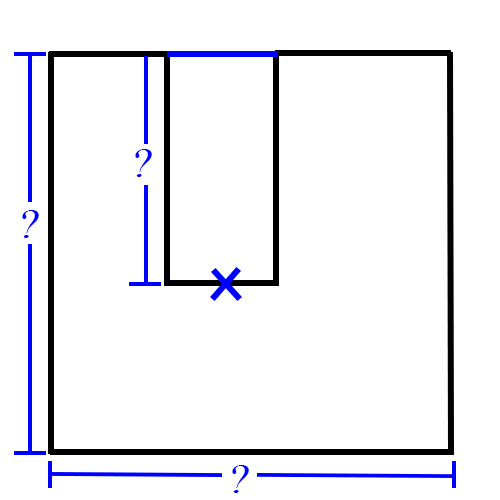
\includegraphics[width=0.3\textwidth]{./pics/Chapter_2/seikai_14.png}
            \end{figure}
        }
    \else
        \vspace{1cm}
    \fi
    % 2017年第二十二届“华罗庚金杯”少年数学邀请赛初赛试卷(小中组).doc; B
}

\item {
    【巧求周长·平移】
    {如图, 在两张大小相同的大长方形纸片上, 分别在角和边上各剪下一个大小相同的小正方形.若图\textcircled{2}阴影部分的周长比图\textcircled{1}阴影部分的周长多17厘米, 那么剪下的小正方形周长为\underline{\hbox to 20mm{}} 厘米.} \\
    \begin{figure}[H] 
        \centering
        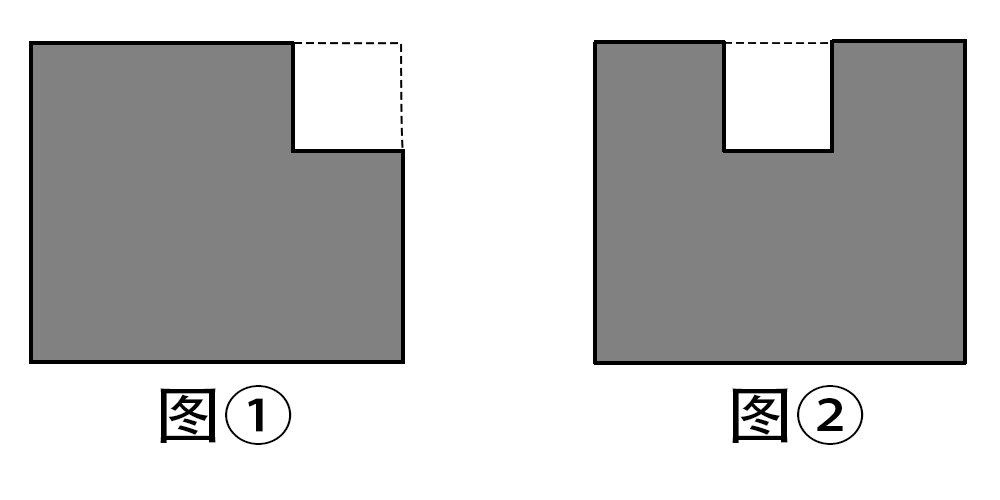
\includegraphics[width=0.5\textwidth]{./pics/Chapter_2/15.png}
    \end{figure}
    \ifshowSolution 
        \fangsong\zihao{5}\textcolor{blue}{
            正解: 34.\\
        }
    \else
        \vspace{1cm}
    \fi
    % 华杯2017; 34
}


\item {
    【三角形面积·完全平方数】
    如图, 将一个正方形硬纸片的四个角分别剪去一个等腰直角三角形, 最后剩下一个长方形.正方形边长和三角形直角边长都是整数.若剪去部分的总面积为40平方厘米, 则长方形的面积是 \underline{\hbox to 20mm{}} 平方厘米.
    \begin{figure}[H] 
        \centering
        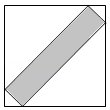
\includegraphics[width=0.3\textwidth]{./pics/Chapter_2/12.png}
    \end{figure}
    \ifshowSolution 
        \fangsong\zihao{5}\textcolor{blue}{
            正解: \\
            2个完全平方数之和为40.\\
            $40 = 2^2 + 6^2$.\\
            $S_{长方形} = 8^2 - 40 = 24 {cm}^2$.
        }
    \else
        \vspace{1cm}
    \fi
    % 2017年第二十二届“华罗庚金杯”少年数学邀请赛决赛试卷(小中组).doc; 24
}

\item {
    【长方形周长·面积】
    如图, 周长为48的大正方形被分成了五个周长相等的长方形, 那么阴影长方形的面积是 \underline{\hbox to 20mm{}}.
    \begin{figure}[H] 
        \centering
        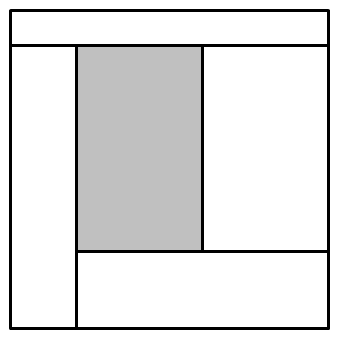
\includegraphics[width=0.2\textwidth]{./pics/Chapter_2/2.png}
    \end{figure}
    \ifshowSolution 
        \fangsong\zihao{5}\textcolor{blue}{
            正解: 40.\\
            \begin{figure}[H] 
                \centering
                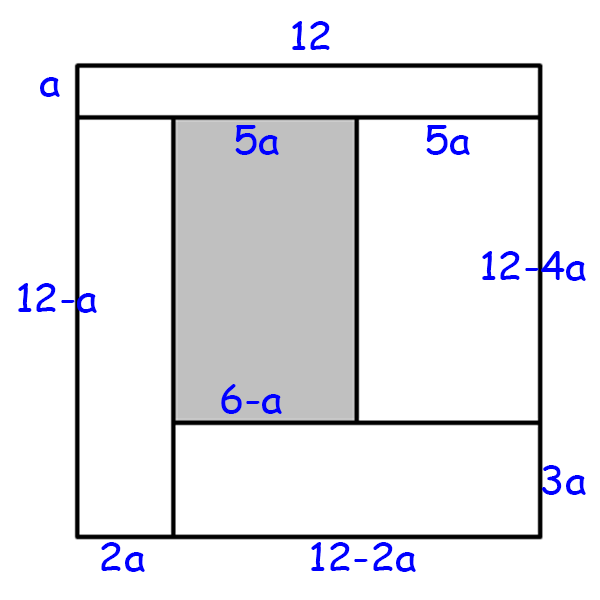
\includegraphics[width=0.3\textwidth]{./pics/Chapter_2/seikai_2.png}
            \end{figure}
            \begin{align*}
                5a &= 6-a \\
                a &= 1 \\
                S_{阴影} &= 5a\cdot (12-4a) \\
                &= 5\times 8\\
                &= 40.
            \end{align*}
        }
    \else
        \vspace{1cm}
    \fi
    % 改. 2024数学花园探秘笔试小中年级夏季决赛C卷(B5试卷版).pdf 
}
\item {
    【长方形周长·面积】
    如图, 一个大正方形被分割成了周长依次为70、80、90、100的四个小长方形;那么, 其中最小的小长方形的面积是\underline{\hbox to 20mm{}}.
    \begin{figure}[H] 
        \centering
        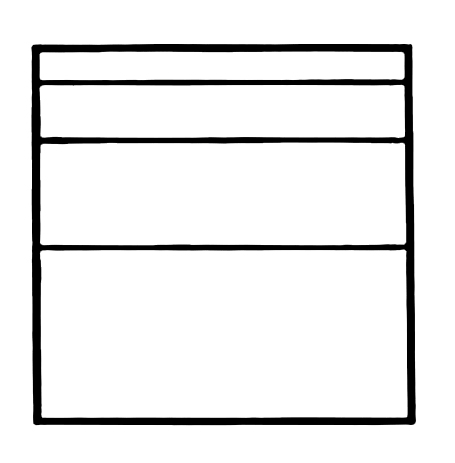
\includegraphics[width=0.3\textwidth]{./pics/Chapter_2/4.png}
    \end{figure}
    \ifshowSolution 
        \fangsong\zihao{5}\textcolor{blue}{
            正解: \\
            方法1. \\
            \begin{figure}[H] 
                \centering
                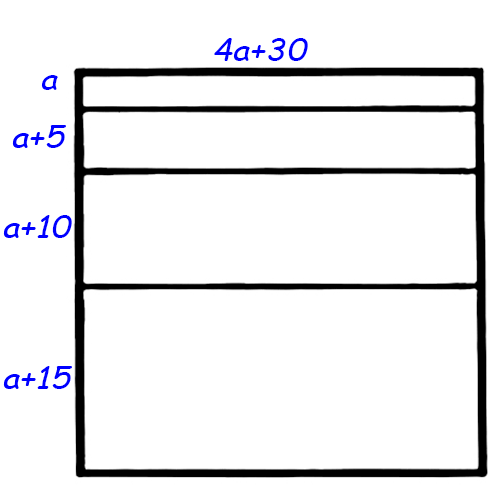
\includegraphics[width=0.3\textwidth]{./pics/Chapter_2/seikai_4.png}
            \end{figure}
            \begin{align*}
                2\times (a+4a+30) &= 70 \\
                a &= 1 \\
                S_{小长方形} &= a\cdot (4a+30)\\
                &= 34.
            \end{align*}
            方法2.\\
            \begin{align*}
                大正方形的边长 &=(70+80+90+100)\div 10 \\
                 &= 34\\
                小长方形的宽 &= 70\div 2 - 34\\
                &= 1\\
                \therefore S_{小长方形} &= 1\times 34\\
                &= 34.
            \end{align*}
        }
    \else
        \vspace{1cm}
    \fi
    % 2023YCB初赛真题答案小中.pdf, 34
}

\item {
    【长方形周长】
    如图中7个小正方形拼成一个大长方形. 如果最小正方形的边长是1, 那么这个大长方形的周长是\underline{\hbox to 20mm{}}.
    \begin{figure}[H] 
        \centering
        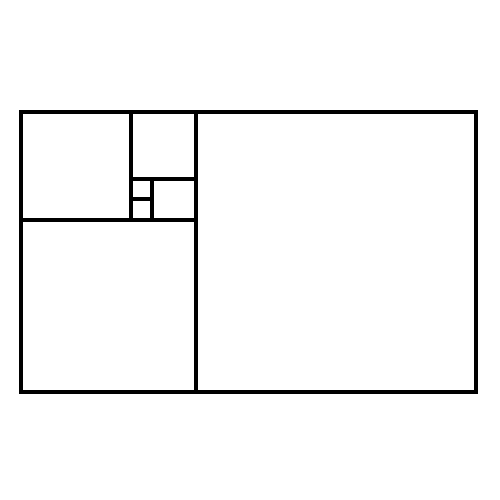
\includegraphics[width=0.4\textwidth]{./pics/Chapter_2/20.png}
    \end{figure}
    \ifshowSolution 
        \fangsong\zihao{5}\textcolor{blue}{
            正解: \\
            \begin{figure}[H] 
                \centering
                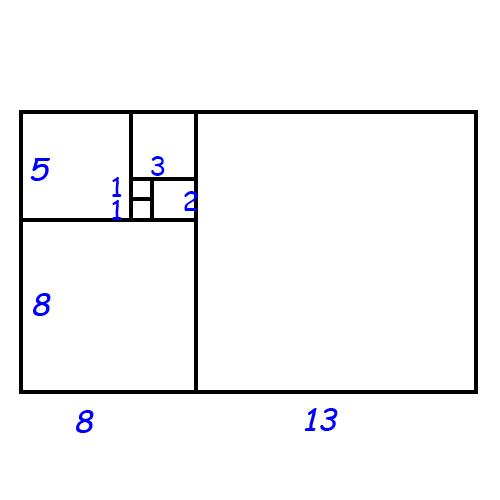
\includegraphics[width=0.4\textwidth]{./pics/Chapter_2/seikai_20.png}
            \end{figure}
            \begin{align*}
                C_{大长方形} &= 2\times (5+8+8+13)\\
                &= 68.
            \end{align*}
        }
    \else
        \vspace{1cm}
    \fi
    % 2015年“迎春杯”数学花园探秘科普活动试卷(小中组决赛a卷).doc; 68
}

\item {
    【图形拼接】
    在一个长方形纸片的左下角剪掉一个小长方形, 再切成三块,  这三块恰好可以拼成一个三角形, 若长方形的宽为12, AB的长度是CD的5倍, 那么EC的长度为\underline{\hbox to 20mm{}}.
    \begin{figure}[H] 
        \centering
        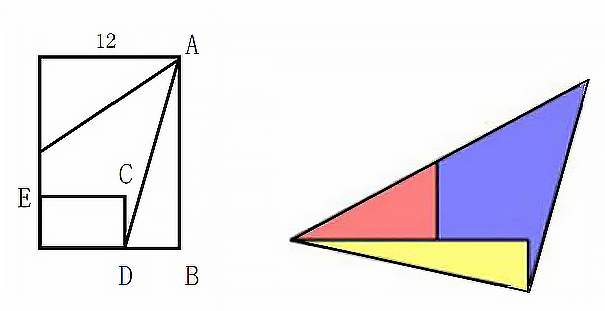
\includegraphics[width=0.6\textwidth]{./pics/Chapter_2/6.png}
    \end{figure}
    \ifshowSolution 
        \fangsong\zihao{5}\textcolor{blue}{
            正解: \\
            设$CD=a$,则$AB=5a$.
            由右图可知, $BD=CD=a$. \\
            在左图中,可得 $CE = 12-BD = 12-a$.\\
            在右图中,可得 $CE = AB-12=5a-12$.\\
            \begin{align*}
                12-a &= 5a-12 ,\\
                a &= 4,\\
                \therefore CE &= 12-a=8.
            \end{align*}
        }
    \else
        \vspace{1cm}
    \fi
    % 8
}

\item {
    【三角形面积·等差数列】
    如图, 一个面积为420平方厘米的长方形被四条线段分割成了五个三角形, 且这五个三角形的面积$S_1, S_2, S_3, S_4, S_5$依次构成等差数列, 那么$S_5$是\underline{\hbox to 20mm{}}平方厘米.
    \begin{figure}[H] 
        \centering
        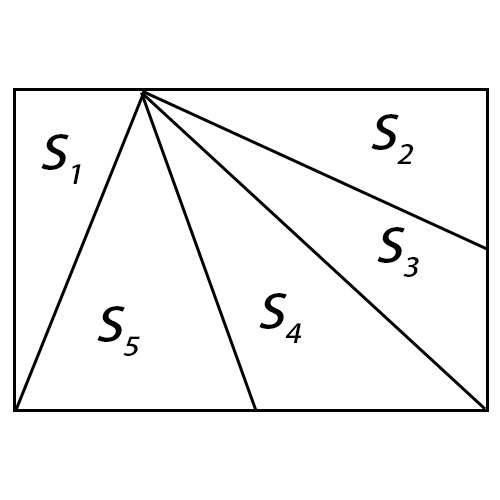
\includegraphics[width=0.4\textwidth]{./pics/Chapter_2/16.png}
    \end{figure}
    \ifshowSolution 
        \fangsong\zihao{5}\textcolor{blue}{
            正解: \\
            方法1(方程).\\
            设公差为d, 则 
            \begin{align*}
                5S_{5} - \frac{5\times 4}{2}d &= 420, \\
                S_{5} - 2d &= 84, \textcircled{1} \\
                S_{4} + S_{5} &= 210, \\
                2S_{5} - d &= 210, \textcircled{2} \\
            \end{align*}
            解方程组
                $\begin{cases}
                    \textcircled{1} \\ 
                    \textcircled{2}  
                \end{cases}$,
            得 $S_{5}=112 {cm}^2$.\\
            方法2.\\
            \begin{align*}
                S_{3} &= 420\div 5 \\
                &= 84 \\
                S_{4} + S_{5} &= 420\div 2\\
                &=210 \\
                \therefore 公差 &= (S_{4} + S_{5} - 2S_{3})\div 3\\
                &= 14\\
                S_{5} &= S_{3} + 14\times 2 \\
                &= 112.
            \end{align*}
        }
    \else
        \vspace{1cm}
    \fi
    % 2016年“迎春杯”数学花园探秘初赛试卷(四年级b卷).doc; 112
}

\item {
    【三角形面积】
    如图中正方形的边长依次是2、4、6、8、10, 阴影部分的面积是\underline{\hbox to 20mm{}}.
    \begin{figure}[H] 
        \centering
        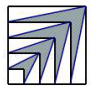
\includegraphics[width=0.3\textwidth]{./pics/Chapter_2/17.png}
    \end{figure}
    \ifshowSolution 
        \fangsong\zihao{5}\textcolor{blue}{
            正解: \\
            方法1.\\
            \begin{align*}
                S_{阴影} &= 10^2 - 2^2 - 2\times \frac12\times (2\times 4 + 2\times 6 + 2\times 8 + 2\times 10) \\
                &= 40.
            \end{align*}
            方法2.\\
            连接对角线.
            \begin{figure}[H] 
                \centering
                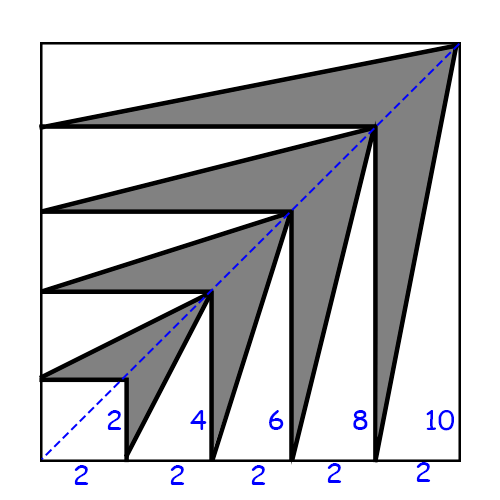
\includegraphics[width=0.3\textwidth]{./pics/Chapter_2/seikai_17.png}
            \end{figure}
            阴影部分由小三角形组成.\\
            $S_{阴影} = 2\times (2\times 2\div 2 + 4\times 2\div 2 + 6\times 2\div 2 + 8\times 2\div 2) = 40.$
        }
    \else
        \vspace{1cm}
    \fi
    % 2016年“迎春杯”数学花园探秘初赛试卷(四年级a卷).doc; 40
}

\item {
    【三角形面积·三角形相似】
    正六边形中如图摆放着两个面积各为30平方厘米的等边三角形, 那么正六边形的面积是\underline{\hbox to 20mm{}}平方厘米.
    \begin{figure}[H] 
        \centering
        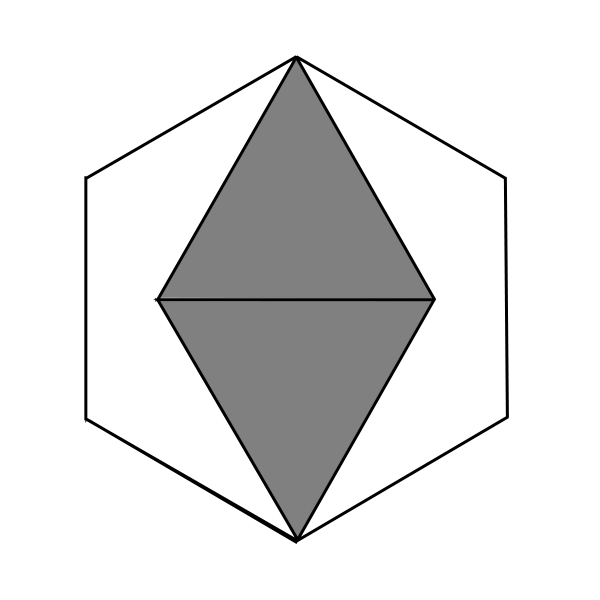
\includegraphics[width=0.4\textwidth]{./pics/Chapter_2/18.png}
    \end{figure}
    \ifshowSolution 
        \fangsong\zihao{5}\textcolor{blue}{
            正解: \\
            方法1(蝴蝶定理).\\
            \begin{figure}[H] 
                \centering
                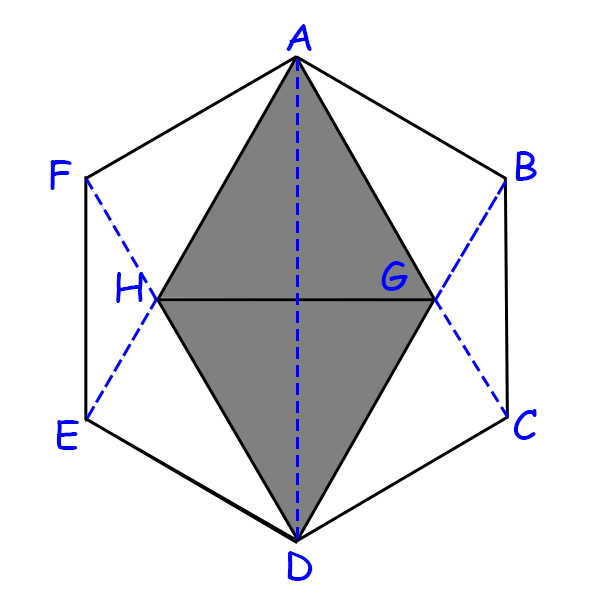
\includegraphics[width=0.4\textwidth]{./pics/Chapter_2/seikai_18.png}
            \end{figure}
            \begin{gather*}
                在梯形ADFE中,S_{\triangle ADH}=30,
                S_{\triangle AFH} = S_{\triangle DEH} = 15. \\
                根据蝴蝶定理,S_{\triangle AFH} \cdot S_{\triangle DEH} = S_{\triangle FEH} \cdot S_{\triangle ADH}\\
                15 \times 15 = S_{\triangle FEH} \cdot 30\\
                S_{\triangle FEH} = \frac{15}{2}\\
                \therefore S_{正六边形} = 2(S_{\triangle EFH} + S_{\triangle AFH} + S_{\triangle ADH}) \\
                = 135 {cm}^2.\\
            \end{gather*}
            方法2(X模型相似).\\
            \begin{gather*}
                根据X模型, \triangle EFH \backsim \triangle ADH, \\
                FH:DH = FH:AH = 1:2, \\
                \therefore S_{\triangle EFH} : S_{\triangle ADH}= 1:4.  \\
                \therefore S_{\triangle EFH}=\frac{15}{2} .\\
                \therefore S_{正六边形} = 2(S_{\triangle EFH} + S_{\triangle AFH} + S_{\triangle ADH}) = 135 {cm}^2.
            \end{gather*}
        }
    \else
        \vspace{1cm}
    \fi
    % 2015年“迎春杯”数学花园探秘科普活动试卷(小中组决赛c卷).doc; 135
}

\item {
    【正方形面积】
    大长方形中如图摆放了四个小正方形, 如果每个小正方形的边长都是6厘米, 那么图中阴影部分的面积是\underline{\hbox to 20mm{}}平方厘米.
    \begin{figure}[H] 
        \centering
        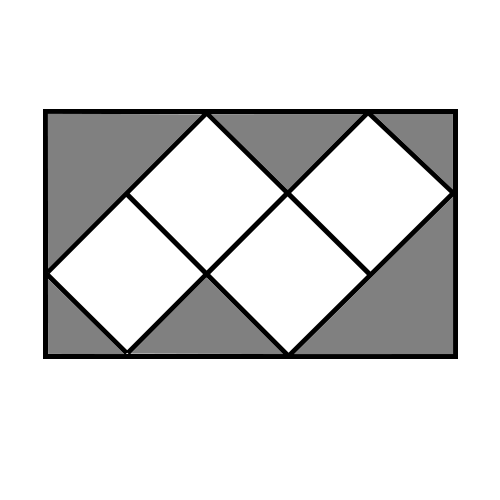
\includegraphics[width=0.4\textwidth]{./pics/Chapter_2/19.png}
    \end{figure}
    \ifshowSolution 
        \fangsong\zihao{5}\textcolor{blue}{
            正解: \\
            \begin{figure}[H] 
                \centering
                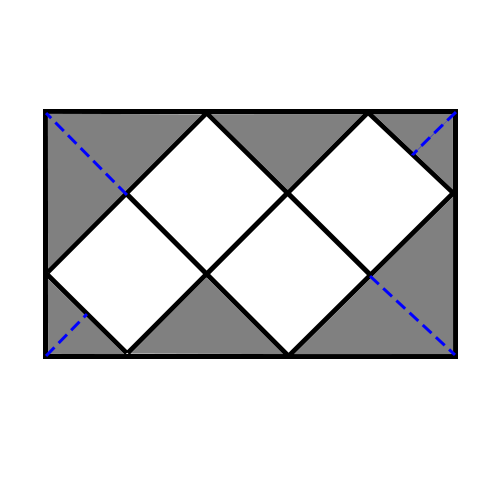
\includegraphics[width=0.4\textwidth]{./pics/Chapter_2/seikai_19.png}
            \end{figure}
            $S_{阴影} = 126 {cm}^2$.
        }
    \else
        \vspace{1cm}
    \fi
    % 2015年“迎春杯”数学花园探秘科普活动试卷(小中组决赛b卷).doc; 126
}

\item {
    【平行四边形面积·等腰直角三角形】
    如图所示, 一个正方形纸片ABCD沿对角线BD剪成两个三角形.第一步操作, 将三角形ABD竖直向下平移3厘米至三角形EFG;第二步操作, 将三角形EFG竖直向下再平移5厘米至三角形HIJ.第一步操作后两张纸片重叠的面积与第二步操作后两张纸片重叠的面积相等, 那么这个正方形纸片ABCD的面积是\underline{\hbox to 20mm{}} 平方厘米.
    \begin{figure}[H] 
        \centering
        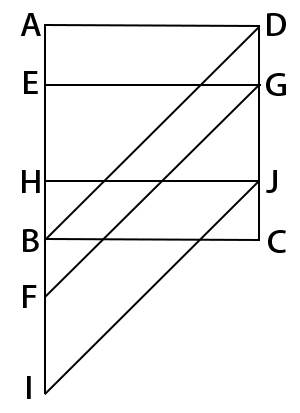
\includegraphics[width=0.3\textwidth]{./pics/Chapter_2/10.png}
    \end{figure}
    \ifshowSolution 
        \fangsong\zihao{5}\textcolor{blue}{
            正解: \\
            \begin{figure}[H] 
                \centering
                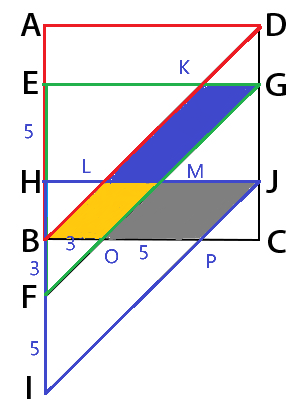
\includegraphics[width=0.3\textwidth]{./pics/Chapter_2/seikai_10.png}
            \end{figure}
            \begin{gather*}
                S_{KLMG} = 3\times 5 = 15, \\
                S_{MOPJ} = OP\cdot JC, \\
                = 5JC, \\
                S_{KLMG} = S_{MOPJ},\\
                \therefore JC = 3 = PC.\\
                S_{正方形ABCD} = (3+5+3)^2 = 121 {cm}^2.\\
            \end{gather*}
        }
    \else
        \vspace{1cm}
    \fi
    % 2018年第二十三届“华罗庚金杯”少年数学邀请赛初赛试卷(小中组).doc; 121
}

\item {
    【三角形相似】
    两个完全一样的长方形如图摆放, 如果整个图形的面积是 420平方厘米, 那么阴影部分的面积是\underline{\hbox to 20mm{}}平方厘米.
    \begin{figure}[H]
        \centering
        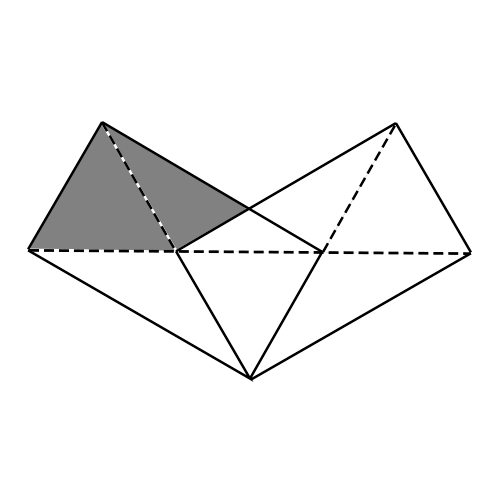
\includegraphics[width=0.4\textwidth]{./pics/Chapter_2/5.png}
    \end{figure}
    \ifshowSolution 
        \fangsong\zihao{5}\textcolor{blue}{
            正解: \\
            $105 {cm}^2$. 
            \begin{figure}[H]
                \centering
                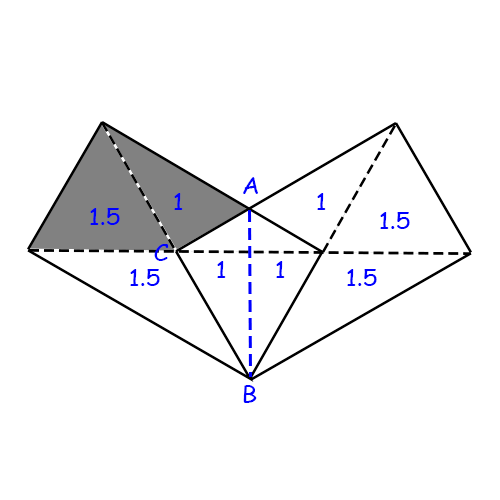
\includegraphics[width=0.4\textwidth]{./pics/Chapter_2/seikai_5.png}
            \end{figure}
            连接辅助线. 设ABC的面积为1份,那么其他部分的份数如图所示.\\
            \begin{align*}
                S_{阴影} &= 420\div 10 \times 2.5 \\
                &= 105 {cm}^2.
            \end{align*}
        }
    \else
        \vspace{1cm}
    \fi
    % 2023改, 105 ; YCB第40届小中组试卷答案.pdf, 84
}

\item {
    【三角形相似·三角形面积】
    如图所示, 两个边长为6的正方形$ABFE$和$CDEF$拼成长方形$ABCD$. G为DE的中点.连接BG交EF于H. 求图中五边形$CDGHF$的面积.
    \begin{figure}[H] 
        \centering
        
\includegraphics[width=0.4\textwidth]{./pics/Chapter_2/13.png}
    \end{figure}
    \ifshowSolution 
        \fangsong\zihao{5}\textcolor{blue}{
            正解: \\
            G为DE的中点,\\
            \begin{align*}
                根据X模型, \triangle HEG \backsim \triangle HFB, \\
                EH:FH = EG:BF = 1:2, \\
                \therefore EH=2, \\
                S_{\triangle HEG} = \frac{1}{2}EH\cdot EG = 3, \\
                S_{阴影} = 36 - 3 = 33.
            \end{align*}
        }
    \else
        \vspace{1cm}
    \fi
    % 2017年第二十二届“华罗庚金杯”少年数学邀请赛决赛试卷(小中组).doc; 33
}

\item {
    【三角形内角和】
    {在下图中, $\angle 1 + \angle 2 + \angle 3 + \angle 4 - \angle 5=$ \underline{\hbox to 20mm{}} $\degree$.} 
    \begin{figure}[H] 
        \centering
        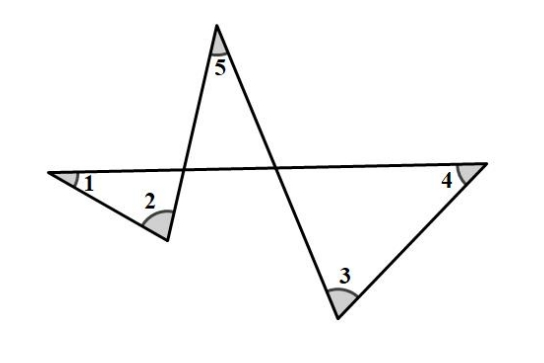
\includegraphics[width=0.4\textwidth]{./pics/Chapter_2/9.png}
    \end{figure}
    \ifshowSolution 
        \fangsong\zihao{5}\textcolor{blue}{
            正解: $180\degree$. \\
        }
    \else
        \vspace{1cm}
    \fi
    % 华数真题2021-2023(小中组).pdf
}

\item {
    【四边形内角和】
    从四边形4个内角取2个求和, 共有6个和数, 则大于$180\degree$的和最多有 \underline{\hbox to 20mm{}} 个.
    \begin{figure}[H] 
        \centering
        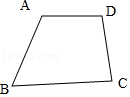
\includegraphics[width=0.4\textwidth]{./pics/Chapter_2/11.png}
    \end{figure}
    \ifshowSolution 
        \fangsong\zihao{5}\textcolor{blue}{
            正解: 3.\\
            设四个角分别是$A,B,C,D$, 则$A+B+C+D = 360\degree$, \\
            6个和为: $A+C, A+B, A+D, B+C, B+D, C+D$. \\
            分三组讨论.\\
            第1组: $A+B, C+D$, $A+B > 180\degree \Rightarrow C+D < 180\degree$, \\
            第2组: $A+C,B+D$, $A+C > 180\degree \Rightarrow B+D < 180\degree$, \\
            第3组: $A+D,C+B$, $A+D > 180\degree \Rightarrow C+B < 180\degree$, \\
            所以, 大于$180\degree$的和最多有 3个.
        }
    \else
        \vspace{1cm}
    \fi
    % 2018年第二十三届“华罗庚金杯”少年数学邀请赛初赛试卷(小中组).doc; 3
}


\item {
    【三角形相似】
    在长方形$ABCD$中, $P,Q$分别是$AD,BC$的中点, $EM\mathop{//}NF\mathop{//}AD$, $AE=CF=5$, 阴影部分面积为50, 那么$AD$的长度为\underline{\hbox to 20mm{}}.
    \begin{figure}[H] 
        \centering
        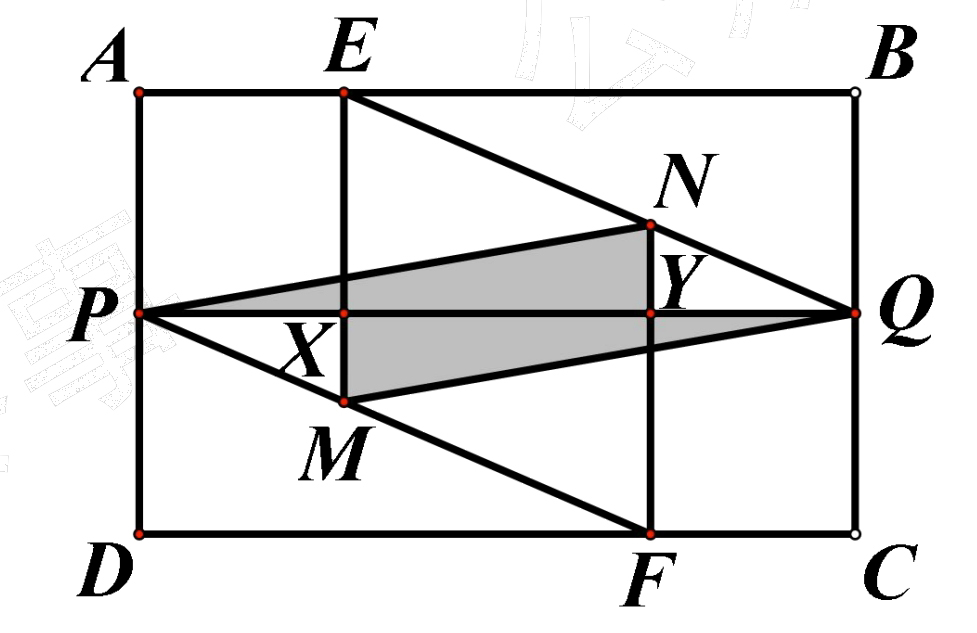
\includegraphics[width=0.4\textwidth]{./pics/Chapter_2/1.png}
    \end{figure}
    \ifshowSolution 
        \fangsong\zihao{5}\textcolor{blue}{
            正解: \\
            设$MX=a, XY =b$.\\
            \begin{align*}
                S_{阴影} &= (5+b)a = 50. \\
                \triangle PMX &\backsim \triangle QEX,\\
                \frac{PX}{MX} &= \frac{QX}{EX}, \\
                \frac{5}{a} &= \frac{5+b}{AP}, \\
                AP &= \frac{(5+b)a}{5} = 10, \\
                AD &= 2AP \\
                &= 20. \\
            \end{align*}
        }
    \else
        \vspace{1cm}
    \fi
    % 17
}


\item {
    【正多边形内角】
    如图所示, 一个正五边形与两个正六边形相邻, 它们的边长相等. 则$\angle ABC = $\underline{\hbox to 20mm{}}.
    \begin{figure}[H] 
        \centering
        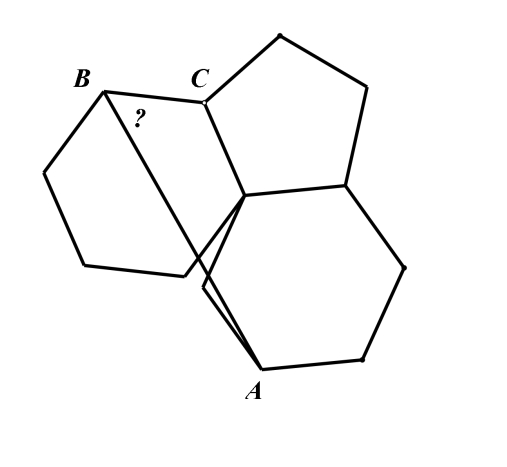
\includegraphics[width=0.4\textwidth]{./pics/Chapter_2/7.png}
    \end{figure}
    \ifshowSolution 
        \fangsong\zihao{5}\textcolor{blue}{
            正解: \\
            $54\degree$.
            \begin{figure}[H] 
                \centering
                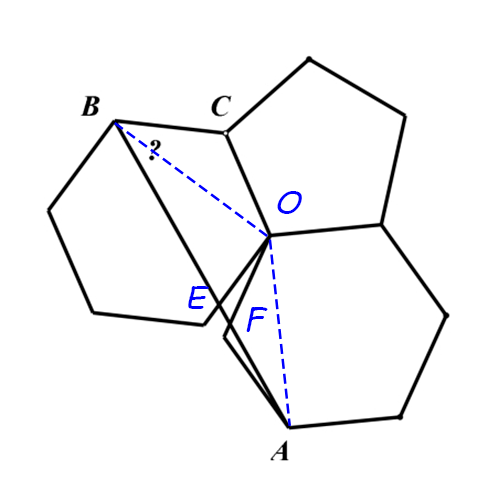
\includegraphics[width=0.4\textwidth]{./pics/Chapter_2/seikai_7.png}
            \end{figure}
            \begin{gather*}
            正五边形一个内角为 108\degree, \\
            正六边形一个内角为120\degree. \\
            连接BO, 容易知道 \angle CBO = 30\degree. \\
            \therefore \angle EOF = 360\degree - 120\degree \times 2 - 108\degree = 12\degree. \\
            在等腰三角形\triangle AOB 中, \\
            \therefore \angle AOB = 120\degree + \angle EOF = 132\degree,\\
            \therefore \angle ABO = (180\degree - 132\degree) \div 2 = 24\degree.\\
            \therefore \angle ABC = 24\degree + 30\degree = 54\degree.\\
            \end{gather*}
        }
    \else
        \vspace{1cm}
    \fi
    % 华数真题2021-2023(小中组).pdf; 
}

\item {
    【正五边形内角·等腰直角三角形】
    如图, 三角形 $ABC$和三角形 $ADE$是 $\angle A=90\degree$ 的等腰直角三角形, 点 $M$ 是 $BC$ 的中点. 已知$AB=AC=DF=FM=EG=GM$, $\angle FDE = \angle GED=9\degree$ 且点$F$和点$G$在三角形$ADE$以外. 问$\angle FMG$ 的度数是\underline{\hbox to 20mm{}}度. 
    \begin{figure}[H] 
        \centering
        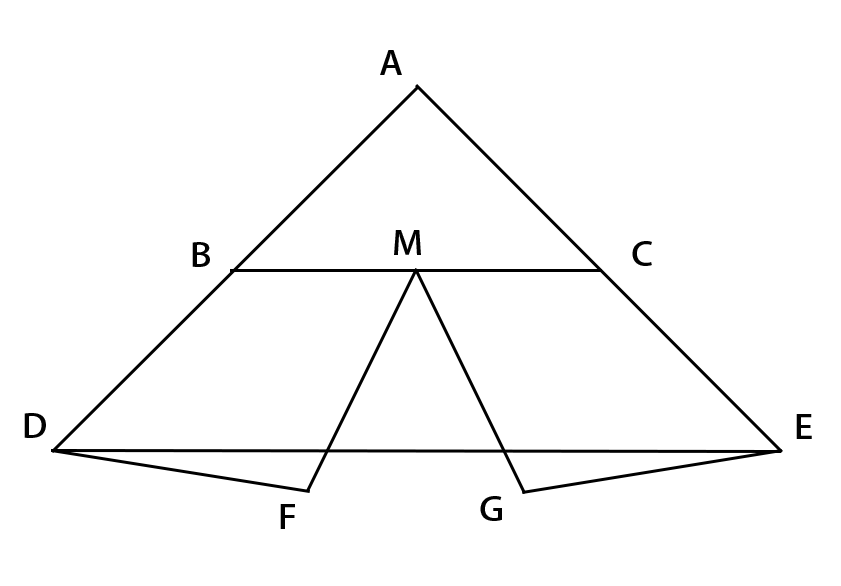
\includegraphics[width=0.4\textwidth]{./pics/Chapter_2/8.png}
    \end{figure}
    \ifshowSolution 
        \fangsong\zihao{5}\textcolor{blue}{
            正解: 54.\\
            如图,构造正方形APBM,作点F关于AD的对称点Q. 连接DQ, PQ, PM.\\
            \begin{figure}[H] 
                \centering
                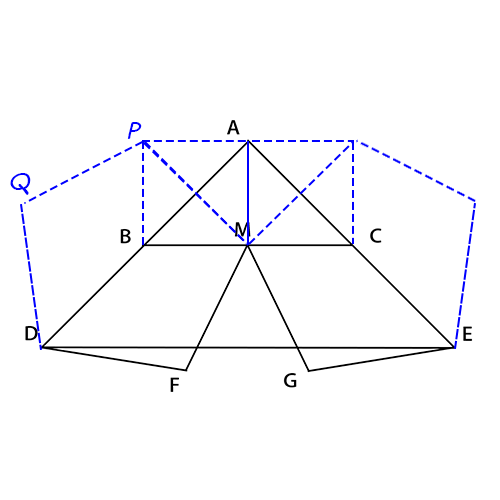
\includegraphics[width=0.4\textwidth]{./pics/Chapter_2/seikai_8.png}
            \end{figure}
            \begin{flalign*}
                &\because 四边形 AMBP 是正方形,\\
                &\therefore PM=AB=MF=FD=DQ=QP,\\
                &\therefore 五边形 PMFDQ 是正五边形. \\
                & 右边同理.\\
                &\therefore \angle FMG=360\degree - 108\degree \times 2 - 90\degree = 54\degree.
            \end{flalign*}
        }
    \else
        \vspace{1cm}
    \fi
    % 华数真题2021-2023(小中组).pdf, 2022.2.19线上小中组解析1.pdf; 54
}


% \item {
%     【三角形面积】
%     如图, 正六边形$ABCDEF$中, 以AB为边长向内作正方形$ABGH$, $CG$与$FH$交于点$M$.\\
%     (1) 如果正六边形$ABCDEF$的边长是20, 那么三角形$AFH$的面积是\underline{\hbox to 20mm{}}.\\
%     (2) 如果正六边形$ABCDEF$的面积是24, 那么阴影部分面积之和是\underline{\hbox to 20mm{}}.
%     \begin{figure}[H] 
%         \centering
%         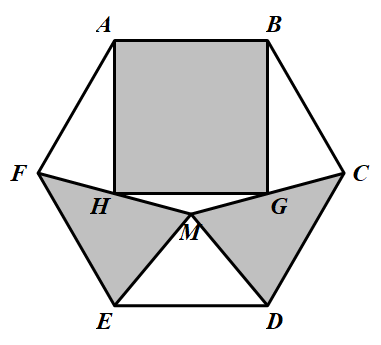
\includegraphics[width=0.4\textwidth]{./pics/Chapter_2/3.png}
%     \end{figure}
%     \ifshowSolution 
%         \fangsong\zihao{5}\textcolor{blue}{
%             正解: \\
%             (1) \\
%             $AB = AF = AH = 20$,\\
%             $\angle FAH = 30\degree,$\\
%             $\therefore \triangle AFH$边 $AF$ 上的高 $h=10$,\\
%             $\therefore S_{\triangle AFH} = \frac12\cdot AF\cdot h = \frac12\times 20\times 10 = 100.$ \\
%             \\(2)\\
%             设 $AB=a.$
%             \begin{align*}
%                 S_{\triangle ABO} &= 4 \\
%                 \frac12\cdot a\cdot \frac{AE}{2} &= 4 \\
%                 a\cdot AE &= 16.\\
%                 S_{\triangle AFH} &= \frac{a^2}{4}. \\
%                 S_{\triangle MHG} + S_{\triangle MDE} &= \frac{1}{2}HG\cdot EH \\
%                 &= \frac{a}{2}\cdot (AE-a). \\
%                 S_{阴影} &= S_{ABCDEF} - 2S_{\triangle AFH} - S_{\triangle MHG} - S_{\triangle MDE} \\
%                 &= 24 - \frac{a^2}{2} - \frac{1}{2}a\cdot AE + \frac{a^2}{2} \\
%                 &= 16.
%             \end{align*}
%         }
%     \else
%         \vspace{1cm}
%     \fi
%     % 2024数学花园探秘笔试小中年级夏季决赛C卷(B5试卷版).pdf
% }